% Options for packages loaded elsewhere
\PassOptionsToPackage{unicode}{hyperref}
\PassOptionsToPackage{hyphens}{url}
%
\documentclass[
]{book}
\usepackage{lmodern}
\usepackage{amsmath}
\usepackage{ifxetex,ifluatex}
\ifnum 0\ifxetex 1\fi\ifluatex 1\fi=0 % if pdftex
  \usepackage[T1]{fontenc}
  \usepackage[utf8]{inputenc}
  \usepackage{textcomp} % provide euro and other symbols
  \usepackage{amssymb}
\else % if luatex or xetex
  \usepackage{unicode-math}
  \defaultfontfeatures{Scale=MatchLowercase}
  \defaultfontfeatures[\rmfamily]{Ligatures=TeX,Scale=1}
\fi
% Use upquote if available, for straight quotes in verbatim environments
\IfFileExists{upquote.sty}{\usepackage{upquote}}{}
\IfFileExists{microtype.sty}{% use microtype if available
  \usepackage[]{microtype}
  \UseMicrotypeSet[protrusion]{basicmath} % disable protrusion for tt fonts
}{}
\makeatletter
\@ifundefined{KOMAClassName}{% if non-KOMA class
  \IfFileExists{parskip.sty}{%
    \usepackage{parskip}
  }{% else
    \setlength{\parindent}{0pt}
    \setlength{\parskip}{6pt plus 2pt minus 1pt}}
}{% if KOMA class
  \KOMAoptions{parskip=half}}
\makeatother
\usepackage{xcolor}
\IfFileExists{xurl.sty}{\usepackage{xurl}}{} % add URL line breaks if available
\IfFileExists{bookmark.sty}{\usepackage{bookmark}}{\usepackage{hyperref}}
\hypersetup{
  pdftitle={Conheça o R: Introdução, dicas e curiosidades},
  pdfauthor={Gabriel Danilo Shimizu},
  hidelinks,
  pdfcreator={LaTeX via pandoc}}
\urlstyle{same} % disable monospaced font for URLs
\usepackage{color}
\usepackage{fancyvrb}
\newcommand{\VerbBar}{|}
\newcommand{\VERB}{\Verb[commandchars=\\\{\}]}
\DefineVerbatimEnvironment{Highlighting}{Verbatim}{commandchars=\\\{\}}
% Add ',fontsize=\small' for more characters per line
\usepackage{framed}
\definecolor{shadecolor}{RGB}{248,248,248}
\newenvironment{Shaded}{\begin{snugshade}}{\end{snugshade}}
\newcommand{\AlertTok}[1]{\textcolor[rgb]{0.94,0.16,0.16}{#1}}
\newcommand{\AnnotationTok}[1]{\textcolor[rgb]{0.56,0.35,0.01}{\textbf{\textit{#1}}}}
\newcommand{\AttributeTok}[1]{\textcolor[rgb]{0.77,0.63,0.00}{#1}}
\newcommand{\BaseNTok}[1]{\textcolor[rgb]{0.00,0.00,0.81}{#1}}
\newcommand{\BuiltInTok}[1]{#1}
\newcommand{\CharTok}[1]{\textcolor[rgb]{0.31,0.60,0.02}{#1}}
\newcommand{\CommentTok}[1]{\textcolor[rgb]{0.56,0.35,0.01}{\textit{#1}}}
\newcommand{\CommentVarTok}[1]{\textcolor[rgb]{0.56,0.35,0.01}{\textbf{\textit{#1}}}}
\newcommand{\ConstantTok}[1]{\textcolor[rgb]{0.00,0.00,0.00}{#1}}
\newcommand{\ControlFlowTok}[1]{\textcolor[rgb]{0.13,0.29,0.53}{\textbf{#1}}}
\newcommand{\DataTypeTok}[1]{\textcolor[rgb]{0.13,0.29,0.53}{#1}}
\newcommand{\DecValTok}[1]{\textcolor[rgb]{0.00,0.00,0.81}{#1}}
\newcommand{\DocumentationTok}[1]{\textcolor[rgb]{0.56,0.35,0.01}{\textbf{\textit{#1}}}}
\newcommand{\ErrorTok}[1]{\textcolor[rgb]{0.64,0.00,0.00}{\textbf{#1}}}
\newcommand{\ExtensionTok}[1]{#1}
\newcommand{\FloatTok}[1]{\textcolor[rgb]{0.00,0.00,0.81}{#1}}
\newcommand{\FunctionTok}[1]{\textcolor[rgb]{0.00,0.00,0.00}{#1}}
\newcommand{\ImportTok}[1]{#1}
\newcommand{\InformationTok}[1]{\textcolor[rgb]{0.56,0.35,0.01}{\textbf{\textit{#1}}}}
\newcommand{\KeywordTok}[1]{\textcolor[rgb]{0.13,0.29,0.53}{\textbf{#1}}}
\newcommand{\NormalTok}[1]{#1}
\newcommand{\OperatorTok}[1]{\textcolor[rgb]{0.81,0.36,0.00}{\textbf{#1}}}
\newcommand{\OtherTok}[1]{\textcolor[rgb]{0.56,0.35,0.01}{#1}}
\newcommand{\PreprocessorTok}[1]{\textcolor[rgb]{0.56,0.35,0.01}{\textit{#1}}}
\newcommand{\RegionMarkerTok}[1]{#1}
\newcommand{\SpecialCharTok}[1]{\textcolor[rgb]{0.00,0.00,0.00}{#1}}
\newcommand{\SpecialStringTok}[1]{\textcolor[rgb]{0.31,0.60,0.02}{#1}}
\newcommand{\StringTok}[1]{\textcolor[rgb]{0.31,0.60,0.02}{#1}}
\newcommand{\VariableTok}[1]{\textcolor[rgb]{0.00,0.00,0.00}{#1}}
\newcommand{\VerbatimStringTok}[1]{\textcolor[rgb]{0.31,0.60,0.02}{#1}}
\newcommand{\WarningTok}[1]{\textcolor[rgb]{0.56,0.35,0.01}{\textbf{\textit{#1}}}}
\usepackage{longtable,booktabs}
\usepackage{calc} % for calculating minipage widths
% Correct order of tables after \paragraph or \subparagraph
\usepackage{etoolbox}
\makeatletter
\patchcmd\longtable{\par}{\if@noskipsec\mbox{}\fi\par}{}{}
\makeatother
% Allow footnotes in longtable head/foot
\IfFileExists{footnotehyper.sty}{\usepackage{footnotehyper}}{\usepackage{footnote}}
\makesavenoteenv{longtable}
\usepackage{graphicx}
\makeatletter
\def\maxwidth{\ifdim\Gin@nat@width>\linewidth\linewidth\else\Gin@nat@width\fi}
\def\maxheight{\ifdim\Gin@nat@height>\textheight\textheight\else\Gin@nat@height\fi}
\makeatother
% Scale images if necessary, so that they will not overflow the page
% margins by default, and it is still possible to overwrite the defaults
% using explicit options in \includegraphics[width, height, ...]{}
\setkeys{Gin}{width=\maxwidth,height=\maxheight,keepaspectratio}
% Set default figure placement to htbp
\makeatletter
\def\fps@figure{htbp}
\makeatother
\setlength{\emergencystretch}{3em} % prevent overfull lines
\providecommand{\tightlist}{%
  \setlength{\itemsep}{0pt}\setlength{\parskip}{0pt}}
\setcounter{secnumdepth}{5}
\usepackage{booktabs}
\ifluatex
  \usepackage{selnolig}  % disable illegal ligatures
\fi
\usepackage[]{natbib}
\bibliographystyle{apalike}

\title{Conheça o R: Introdução, dicas e curiosidades}
\author{Gabriel Danilo Shimizu}
\date{2021-03-09}

\begin{document}
\maketitle

{
\setcounter{tocdepth}{1}
\tableofcontents
}
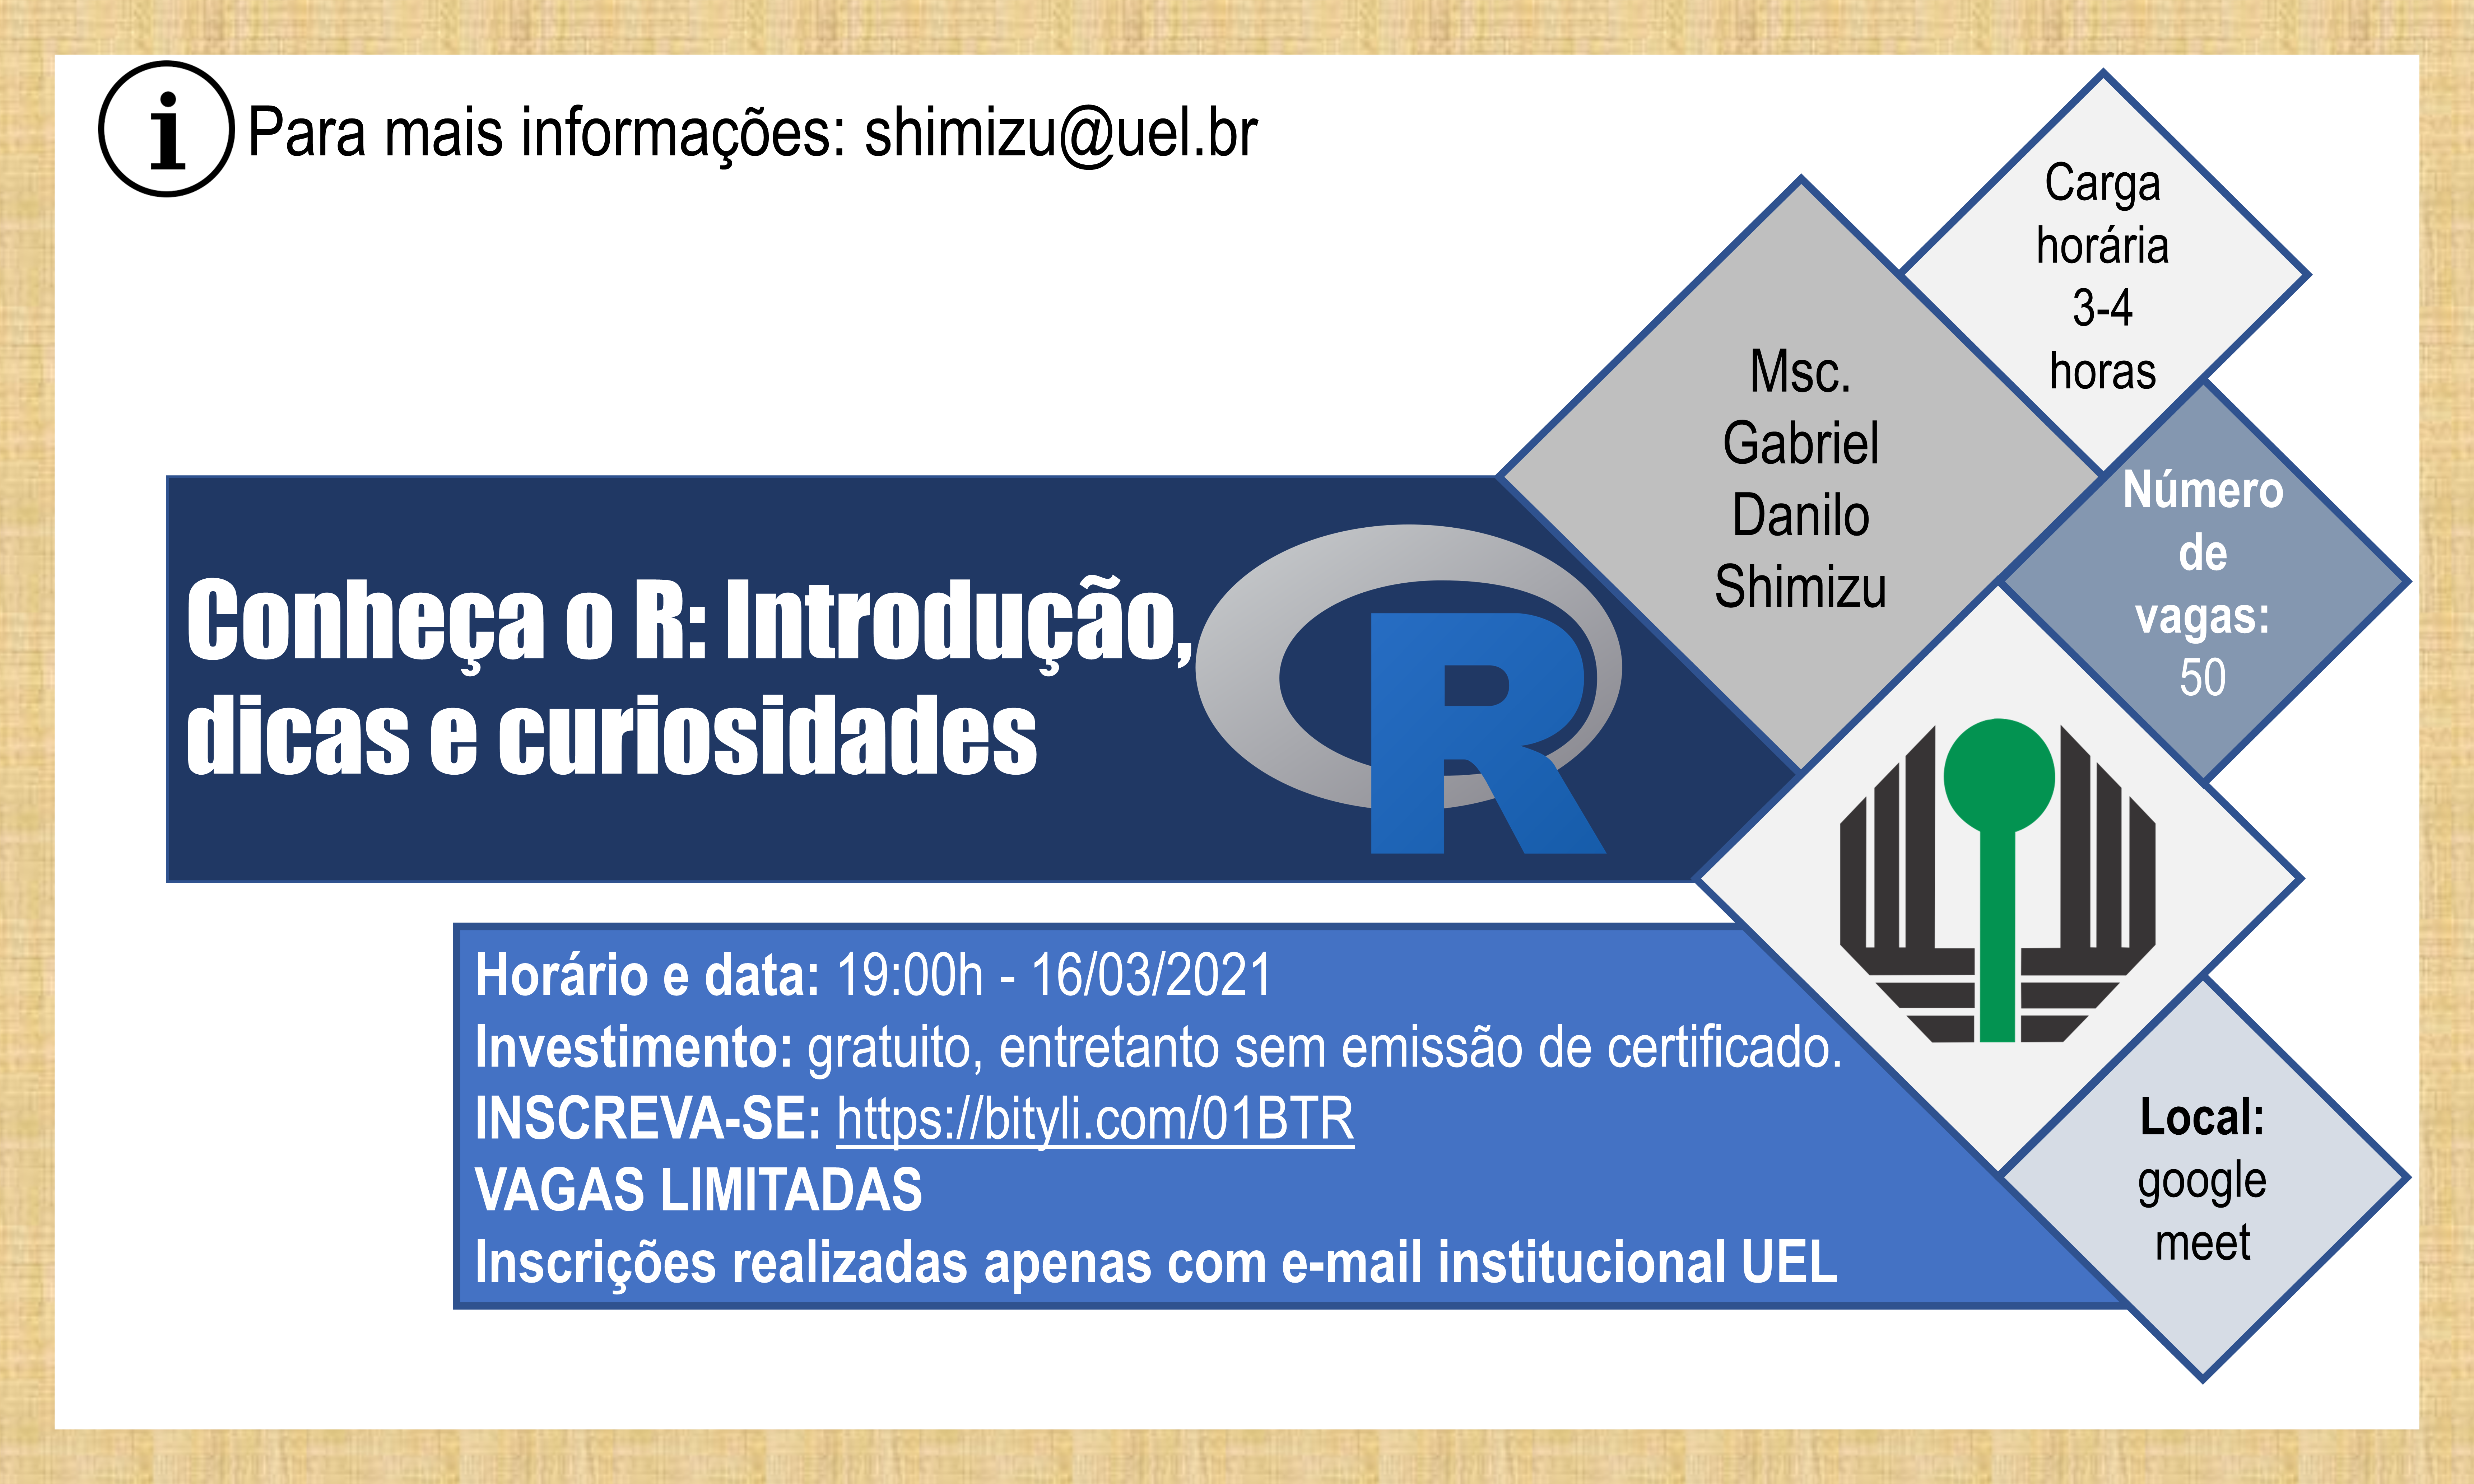
\includegraphics{folder.png}

\hypertarget{conheuxe7a-o-r-introduuxe7uxe3o-dicas-e-curiosidades}{%
\chapter{Conheça o R: Introdução, dicas e curiosidades}\label{conheuxe7a-o-r-introduuxe7uxe3o-dicas-e-curiosidades}}

\emph{Horário e data}: 19:00h - 16/03/2021

\emph{Local}: remoto via google meet

\emph{Carga horária}: de 3 a 4 horas

\emph{Número de vagas}: 50

\emph{Objetivo}: proporcionar um conhecimento mínimo sobre a linguagem R.

\emph{Público alvo}: estudantes de pós-graduação em agronomia.

\emph{Conteúdo}:

\begin{itemize}
\tightlist
\item
  Introdução a linguagem R e ao ambiente Rstudio
\item
  Dicas de importação de dados, geração de gráficos, atalhos, pacotes e informações no geral
\item
  Curiosidades
\end{itemize}

\emph{Investimento}: gratuito, entretanto sem emissão de certificado.

\emph{Ministrante}: Gabriel Danilo Shimizu

VAGAS LIMITADAS: Inscrições realizadas apenas com e-mail institucional UEL

\hypertarget{apresentauxe7uxe3o}{%
\chapter{Apresentação}\label{apresentauxe7uxe3o}}

O R é uma linguagem de programação muito utilizada na âmbito da estatística e na ciência de dados. Na Agronomia, o conhecimento sobre essa linguagem é um diferencial, sobretudo na carreira acadêmica, pois sua limitação gráfica e de análises é praticamente inexistente.

Este curso, embora curto, representa um primeiro passo para os futuros usuários de R e, é essencial para a compreensão das diversas funcionalidades dessa linguagem de programação.

\hypertarget{o-que-uxe9-o-r}{%
\chapter{O que é o R}\label{o-que-uxe9-o-r}}

R é um ambiente computacional e uma linguagem de programação especializada em manipulação, análise e visualização gráfica de dados. Na atualidade é considerado o melhor ambiente computacional para essa finalidade. O ambiente está disponível para diferentes sistemas operacionais: Unix/Linux, Mac e Windows.

Foi criado originalmente por Ross Ihaka e por Robert Gentleman no departamento de Estatística da Universidade de Auckland, Nova Zelândia. Posteriormente, foi desenvolvido pelo esforço colaborativo de pessoas em vários locais do mundo.

O nome R provém em parte das iniciais dos criadores (Ross Ihaka e Robert Gentleman) e também de um jogo figurado com a linguagem S (da Bell Laboratories, antiga AT\&T).

R é um ambiente e uma linguagem de programação similar ao S, contudo, é uma implementação distinta do S. Muitos códigos escritos para o S podem ser executados inalterados no R e vice-versa.

R é altamente expansível com o uso dos pacotes. Os pacotes são bibliotecas com dados e funções para diferentes áreas do conhecimento relacionado a estatística e áreas afins.

Um conjunto básico de pacotes vem embutido na instalação do R, com muito outros disponíveis na rede de distribuição do R (em inglês CRAN).

A linguagem R é largamente usada entre estatísticos e analistas de dados para desenvolver software de estatística e análise de dados. Pesquisas e levantamentos com profissionais da área mostram que a popularidade do R aumentou substancialmente nos últimos anos.

\hypertarget{porque-utilizar-o-r}{%
\section{Porque utilizar o R?}\label{porque-utilizar-o-r}}

\begin{itemize}
\tightlist
\item
  Software gratuito com código aberto com uma linguagem acessível; Expansão exponencial entre pesquisadores, engenheiros e estatísticos;
\item
  Se reinventa constantemente através de novas aplicações (aproximadamente 14.762 pacotes);
\item
  Cobertura inigualável, tecnologia de ponta;
\item
  Totalmente flexível, permitindo desenvolver facilmente funções e pacotes para facilitar o trabalho;
\item
  Capacidade gráfica;
\item
  Disponível para diferentes plataformas: Windows, Linux e Mac.
\end{itemize}

Total de package no CRAN: 17275

Atualizado em: 09/03/2021

(\href{https://cran.r-project.org/web/packages/}{CRAN})

\hypertarget{instalauxe7uxe3o-do-software-r}{%
\chapter{Instalação do software R}\label{instalauxe7uxe3o-do-software-r}}

link para download:

\href{https://www.r-project.org/}{Software R}

\href{https://www.rstudio.com/products/rstudio/download/}{R Studio}

Acessar: \url{https://www.r-project.org/}

Ir em: Download \textgreater{} CRAN

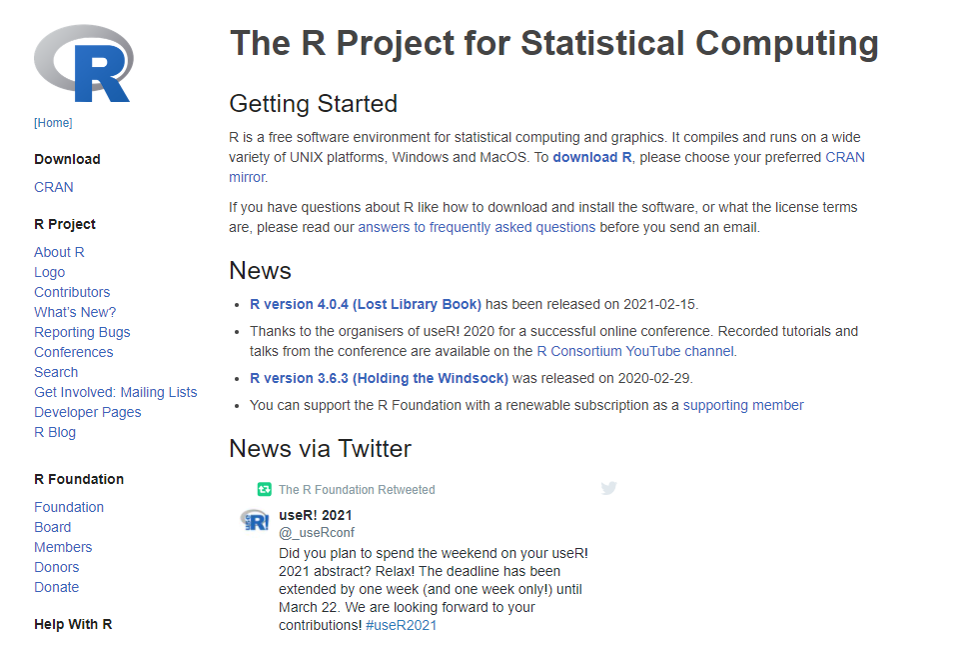
\includegraphics{install1.png}

Ir em: Universidade Federal do Paraná

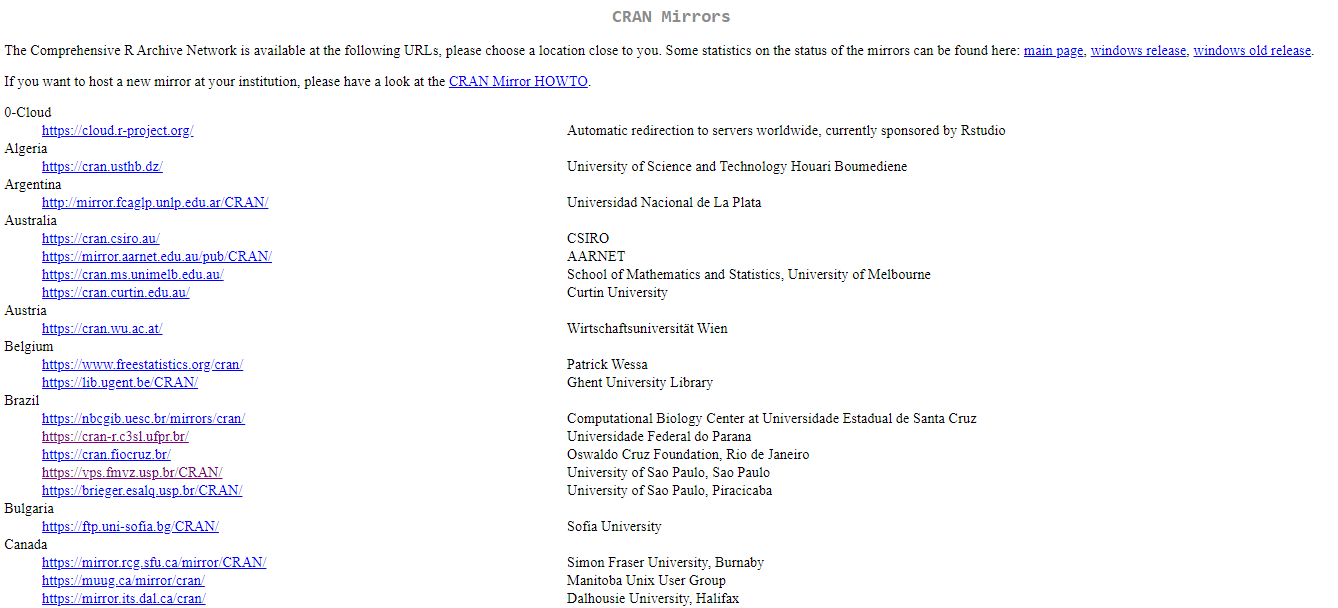
\includegraphics{install2.png}

Ir em: Escolher a opção do sistema operacional do computador

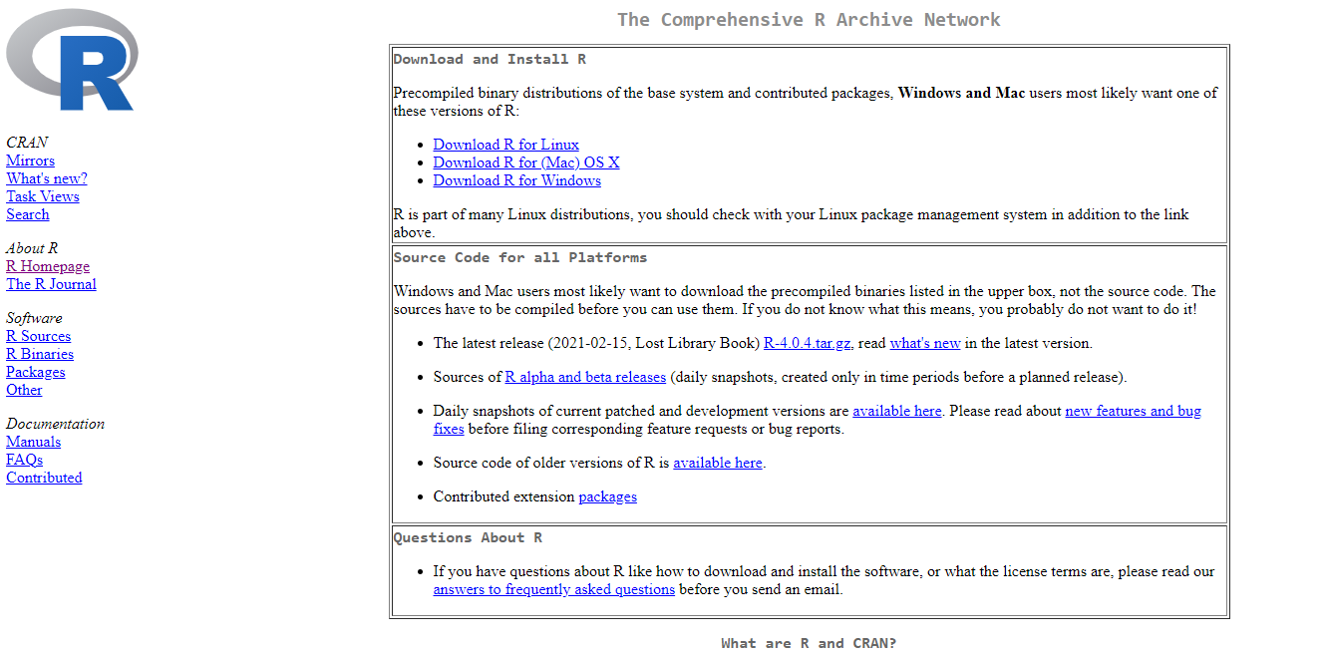
\includegraphics{install3.png}

Ir em: Instalar R pela primeira vez

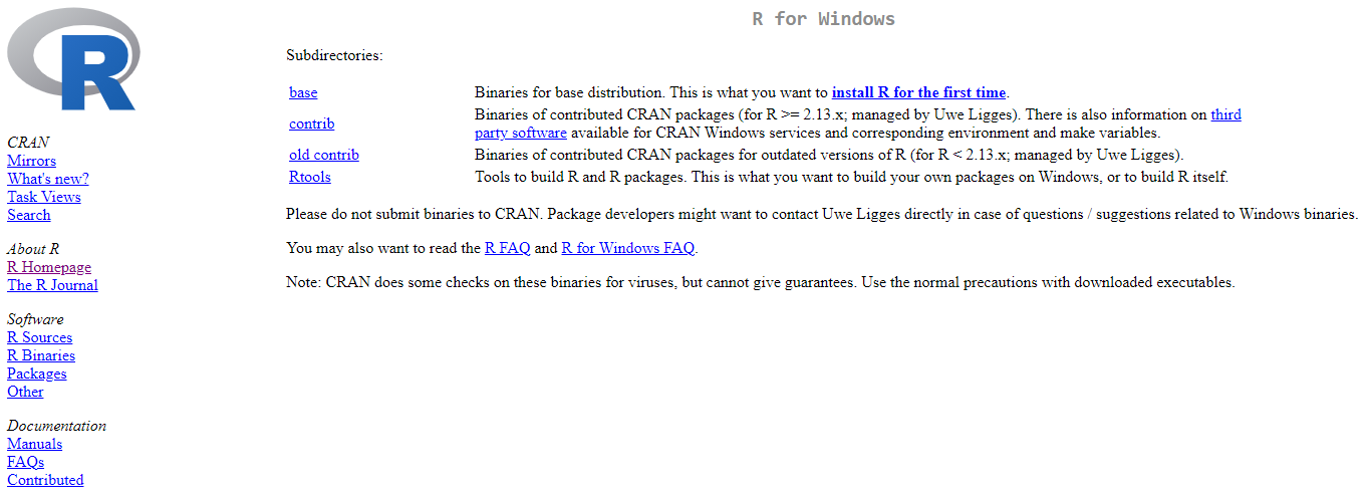
\includegraphics{install4.png}

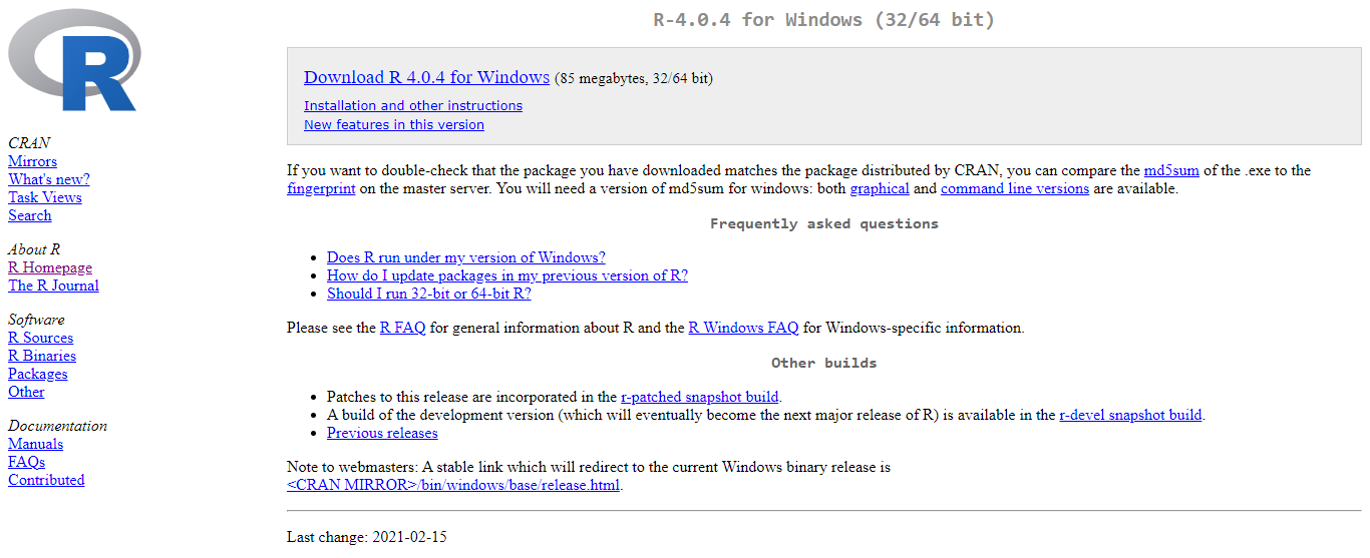
\includegraphics{install5.png}

\href{https://cran.r-project.org/bin/windows/base/old/}{Versões anteriores do R}

Executar o instalador

\hypertarget{instalando-rstudio}{%
\section{Instalando RStudio}\label{instalando-rstudio}}

Acessar: \url{https://www.rstudio.com/}

Ir em: Download


\includegraphics{install6.png}

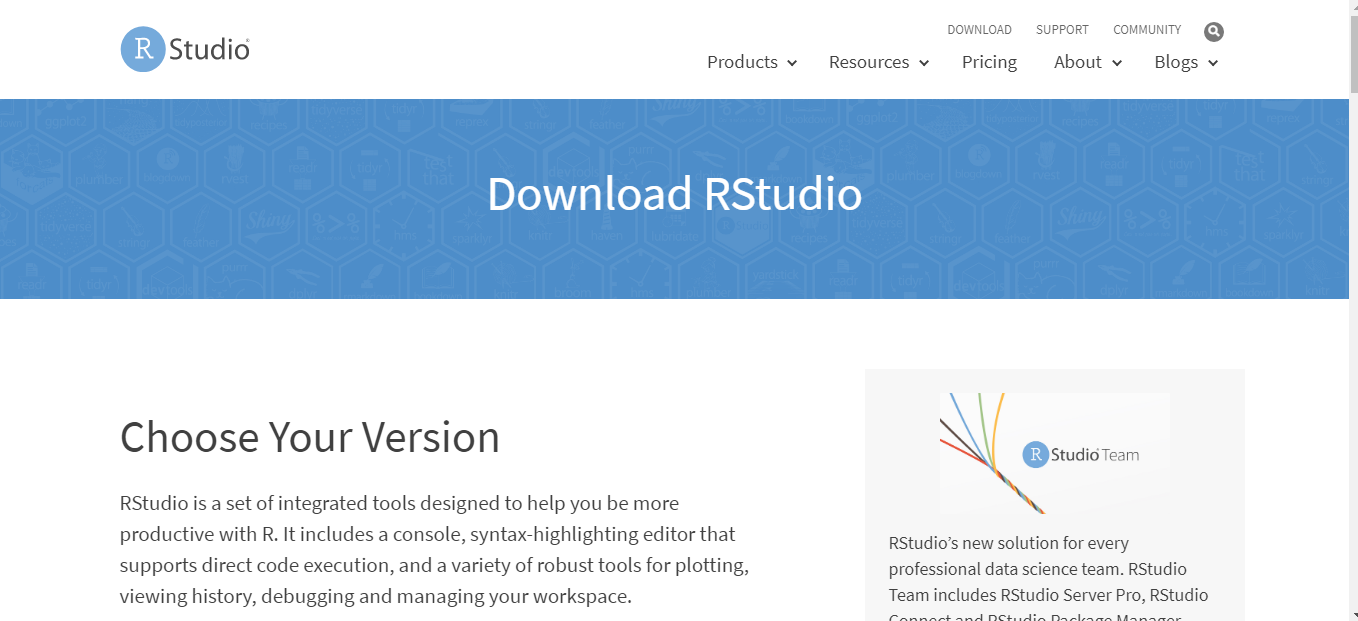
\includegraphics{install7.png}

Baixar a versão do Rstudio correspondente ao seu sistema operacional

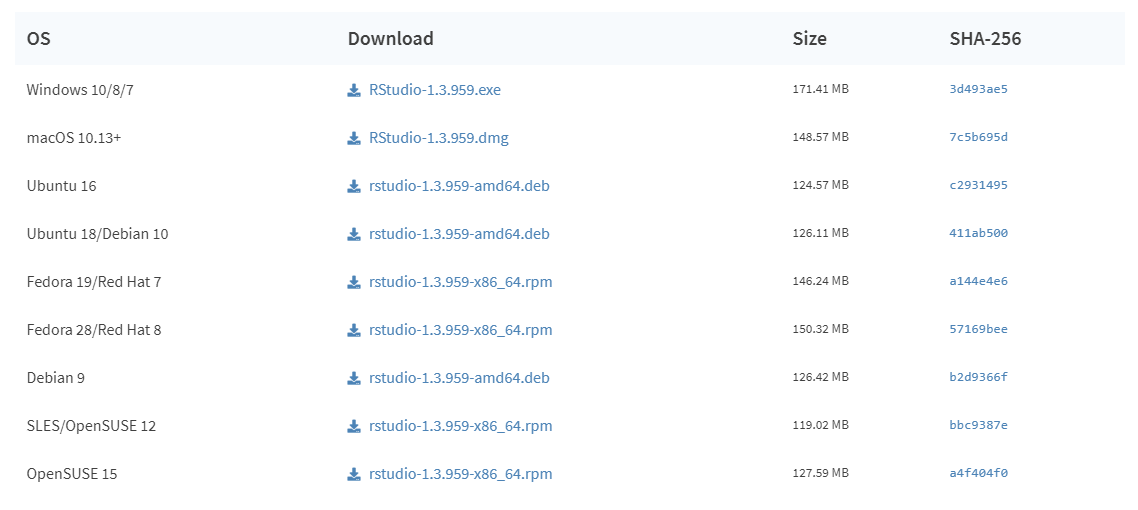
\includegraphics{install8.png}

Executar o instalador.

\hypertarget{primeiros-passos}{%
\section{Primeiros passos}\label{primeiros-passos}}

Abra o Rstudio

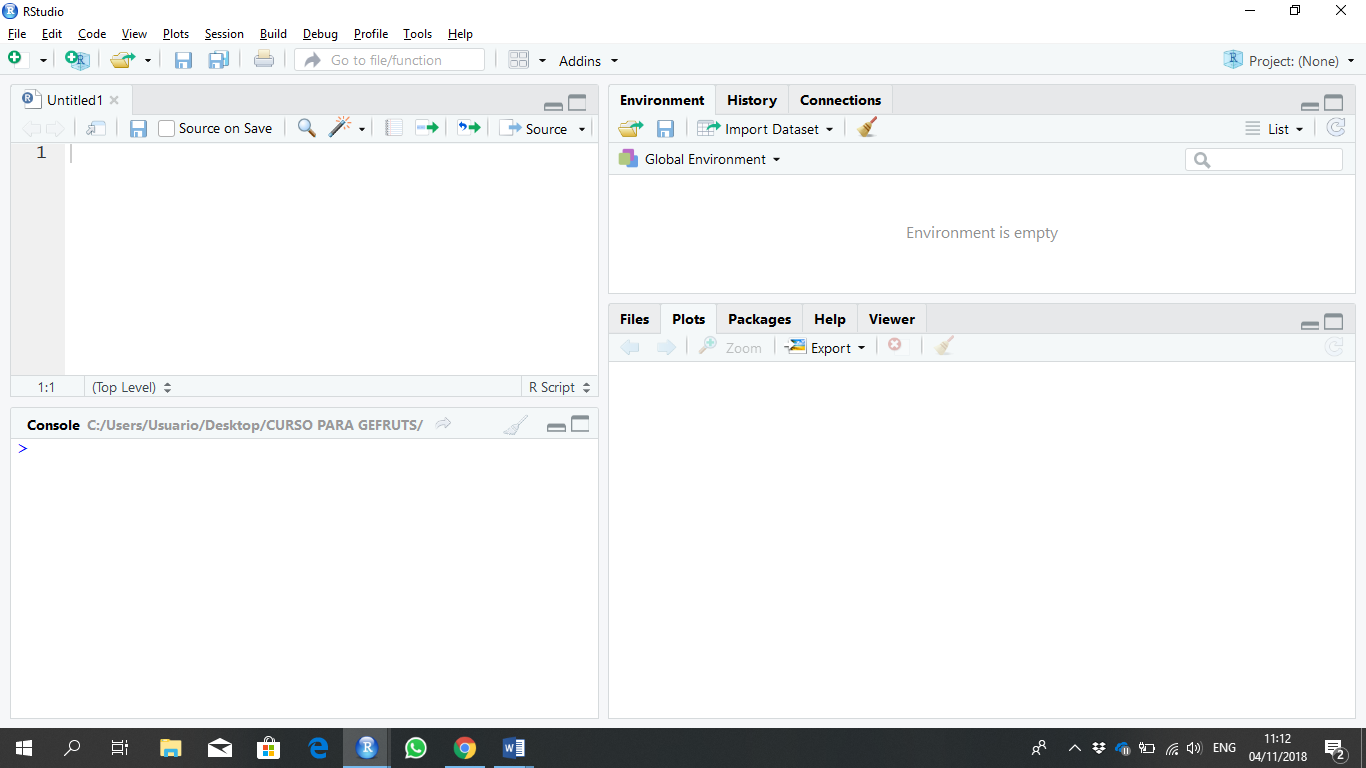
\includegraphics{install9.png}

Ambiente Rstudio

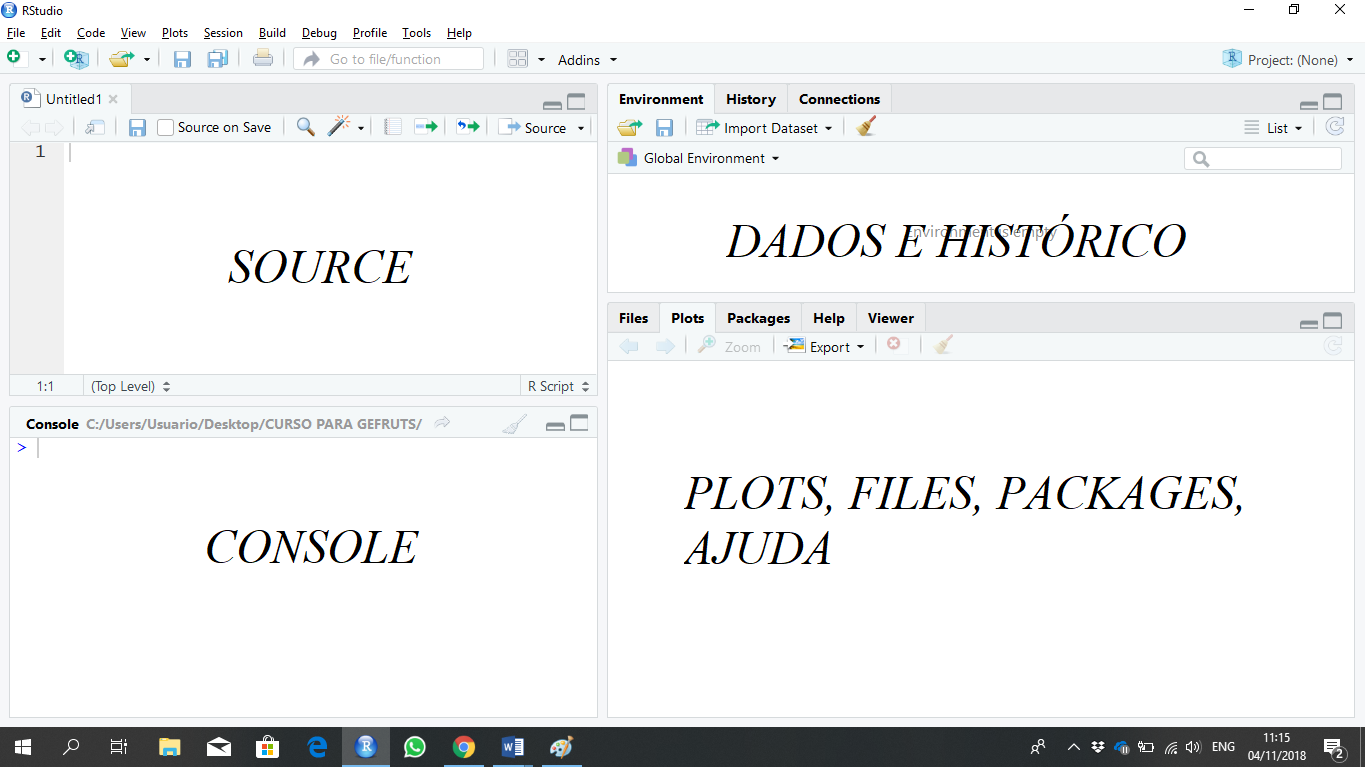
\includegraphics{install10.png}

Source: é seu script (Sempre construir o script aqui, nunca no console)
Console: é a saída
Dados e histórico: é onde está os dados e tudo que foi realizado durante a análise
Plots, files, packages, ajuda: é a saída gráfica, as pastas do diretório atual, os pacotes instalados e a ajuda

\hypertarget{instalando-packages}{%
\section{Instalando packages}\label{instalando-packages}}

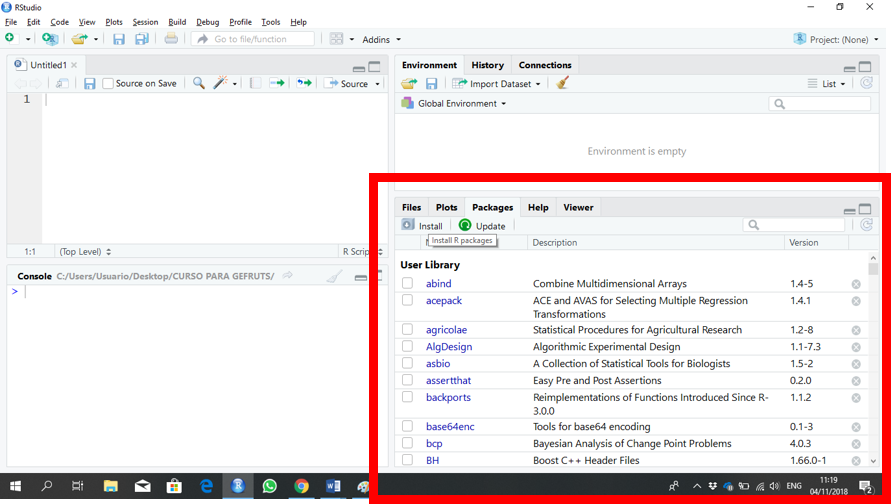
\includegraphics{install11.png}

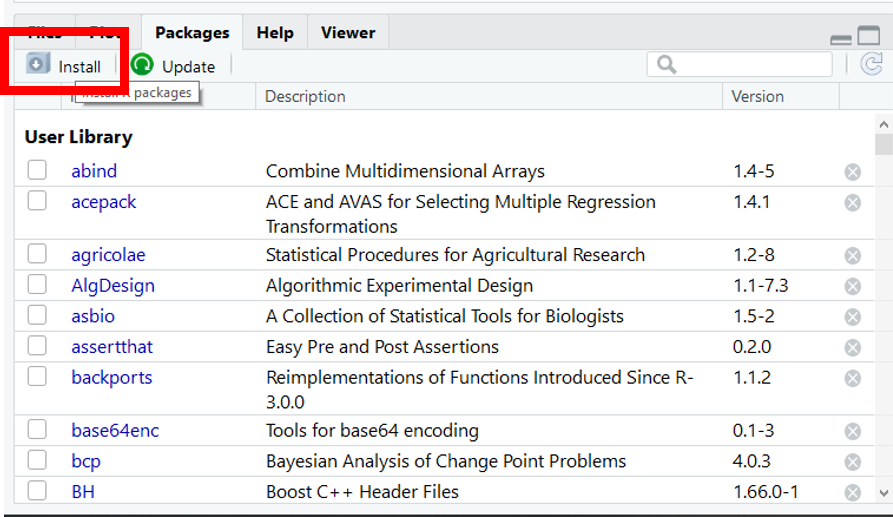
\includegraphics{install12.png}

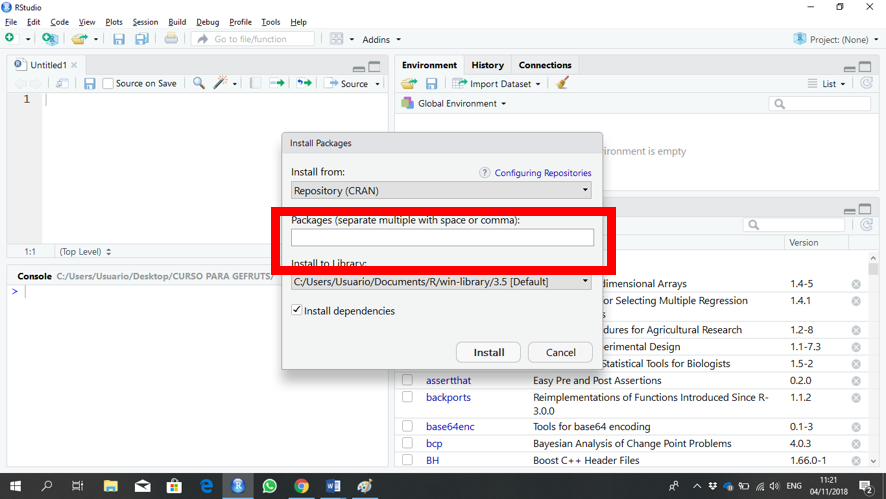
\includegraphics{install13.png}

Digitar o nome do pacote desejado e depois em ``Install''.

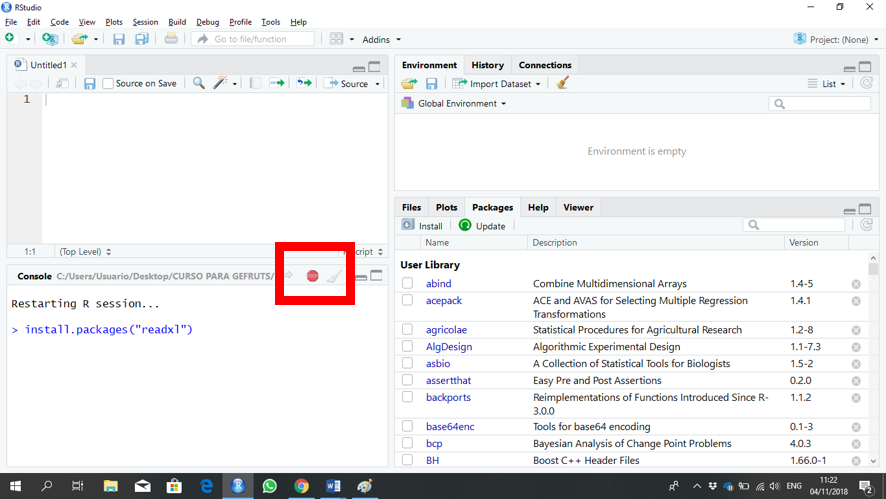
\includegraphics{install16.png}
Toda vez que aparecer o ícone em vermelho, o Rstudio está trabalhando, dessa forma, não executar mais nada até o ícone desaparecer.

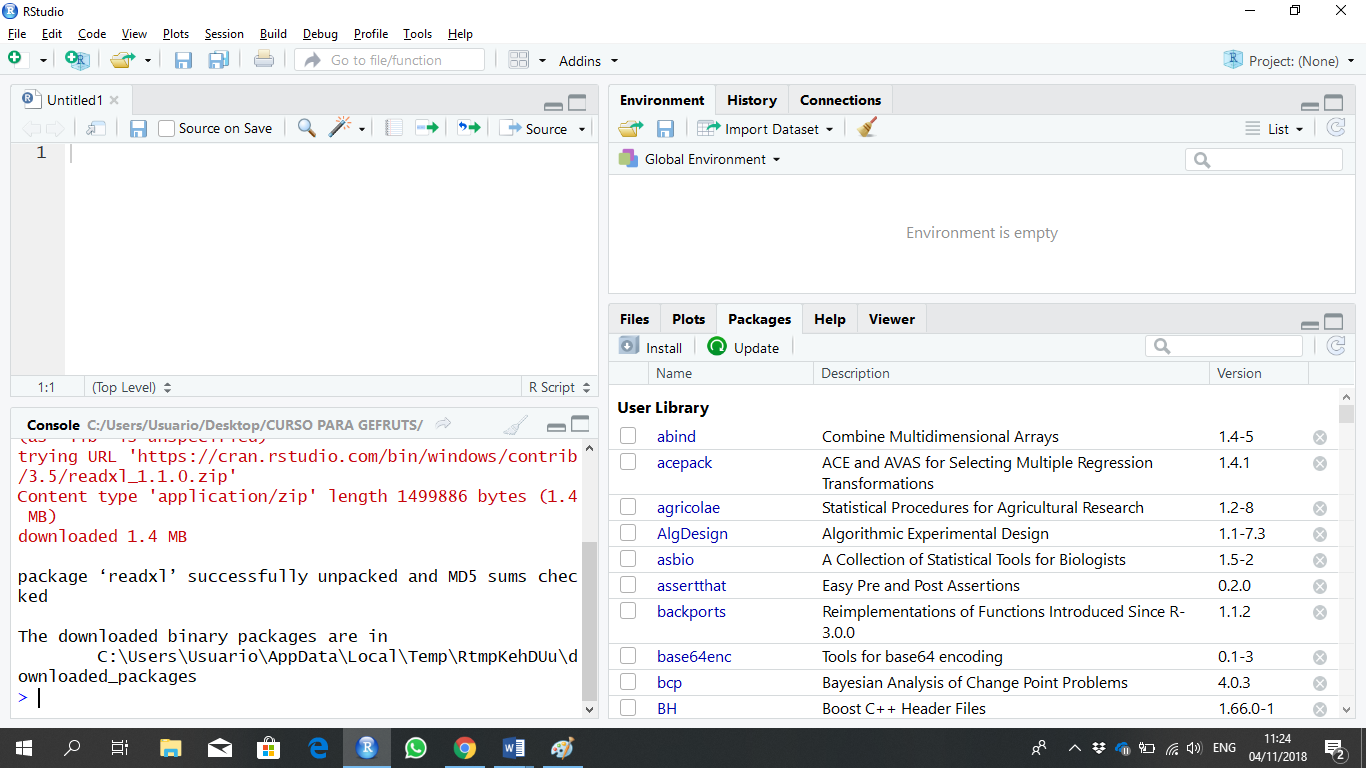
\includegraphics{install15.png}

\hypertarget{chamando-pacote-no-rstudio}{%
\section{Chamando pacote no Rstudio}\label{chamando-pacote-no-rstudio}}

Função:

\texttt{library(nome\ do\ pacote)}
\texttt{require(nome\ do\ pacote)}

nome do pacote::

Ex. library(readxl); require(readxl); readxl::

\hypertarget{importauxe7uxe3o-de-dados}{%
\chapter{Importação de dados}\label{importauxe7uxe3o-de-dados}}

\hypertarget{importauxe7uxe3o-de-dados-do-excel}{%
\section{Importação de dados do excel}\label{importauxe7uxe3o-de-dados-do-excel}}

\href{}{
\includegraphics{excelR.png}}

\hypertarget{utilizando-a-package-readxl}{%
\subsection{Utilizando a package readxl}\label{utilizando-a-package-readxl}}

Existem diversas formas de importação arquivos para o R. Uma das mais utilizadas é a importação de um arquivo em excel.

O excel pode possuir dois tipos de extensão, \textbf{.xls} ou \textbf{.xlsx}, sendo as versões anteriores e superiores ao office 2010, respectivamente.

Uma das packages mais utilizadas para importação os dados de um arquivo em excel é chamado de \textbf{``readxl''}.

Para importar por esse pacote, devemos seguir os passos a seguir:

\hypertarget{especificar-o-diretuxf3rio-onde-fica-o-arquivo-em-excel.}{%
\subsection{Especificar o diretório onde fica o arquivo em excel.}\label{especificar-o-diretuxf3rio-onde-fica-o-arquivo-em-excel.}}

Uma das formas de especificar o diretório buscando a pasta manualmente, como na Figura 1 (copiar e colar no Source do Rstudio).

\begin{figure}
\centering
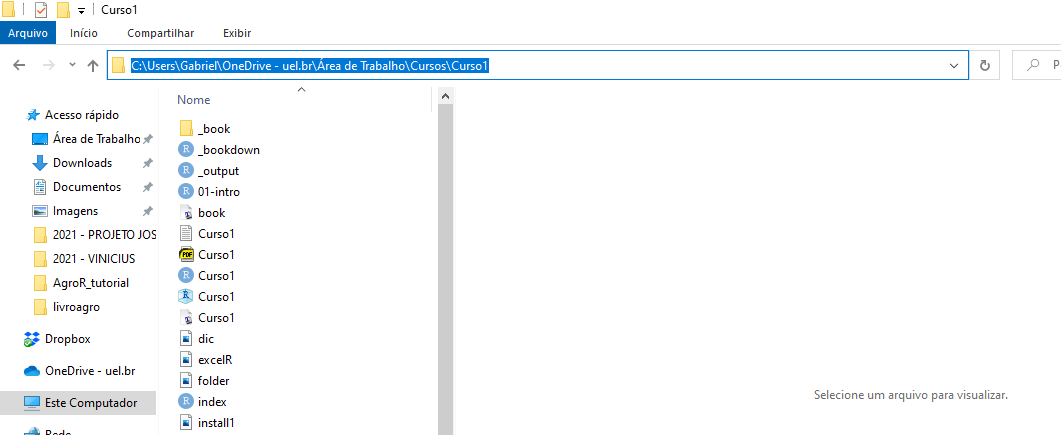
\includegraphics{pasta.png}
\caption{Figura 1: Especificando diretório de trabalho}
\end{figure}

A seguir, é necessário trocar as barras de ~para / ou adicionar mais uma \textbackslash{} (\textbackslash{} para \textbackslash) e colocar dentro do comando setwd e o diretório entre aspas.

Obs. O diretório abaixo é do \textbf{meu computador}!!!

\begin{Shaded}
\begin{Highlighting}[]
\FunctionTok{setwd}\NormalTok{(}\StringTok{"C:}\SpecialCharTok{\textbackslash{}\textbackslash{}}\StringTok{Users}\SpecialCharTok{\textbackslash{}\textbackslash{}}\StringTok{Gabriel Shimizu}\SpecialCharTok{\textbackslash{}\textbackslash{}}\StringTok{Dropbox}\SpecialCharTok{\textbackslash{}\textbackslash{}}\StringTok{ProjetoExperimental}\SpecialCharTok{\textbackslash{}\textbackslash{}}\StringTok{Análise Descritiva"}\NormalTok{)}

\DocumentationTok{\#\# ou}

\FunctionTok{setwd}\NormalTok{(}\StringTok{"C:/Users/Gabriel Shimizu/Dropbox/ProjetoExperimental/Análise Descritiva"}\NormalTok{)}
\end{Highlighting}
\end{Shaded}

Obs. \textbf{Sempre que for alterar a local da pasta, devemos alterar a localização do diretório!!!}

\hypertarget{opuxe7uxe3o-2-para-especificar-diretuxf3rio}{%
\subsection{Opção 2 para especificar diretório}\label{opuxe7uxe3o-2-para-especificar-diretuxf3rio}}

Atalho: ctrl+shift+h

Este comando irá buscar as \textbf{pastas} (não irá aparecer nenhum arquivo a menos que seja uma pasta). Buscar a pasta que contém o arquivo (Deverá saber onde fica, pois por esse método, o arquivo em extensão excel não irá aparecer, uma vez que o excel não é uma pasta)

Após encontrar, clicar em \textbf{``open''}. No console do R irá aparecer \textbf{setwd(localização)}, esta é a localização. Recomendo copiar e colar no \textbf{Source} do Rstudio

\hypertarget{conferir-se-o-arquivo-estuxe1-no-diretuxf3rio-especificado}{%
\subsection{Conferir se o arquivo está no diretório especificado}\label{conferir-se-o-arquivo-estuxe1-no-diretuxf3rio-especificado}}

\begin{Shaded}
\begin{Highlighting}[]
\FunctionTok{dir}\NormalTok{()}
\end{Highlighting}
\end{Shaded}

\hypertarget{ativando-a-package-e-importando-o-arquivo}{%
\subsection{Ativando a package e importando o arquivo}\label{ativando-a-package-e-importando-o-arquivo}}

Antes de ativar o pacote, deve-se instalar o mesmo (Ver guia de instalação - \href{https://agronomiar.000webhostapp.com/manual_instalacao.pdf}{Instalação})

\begin{Shaded}
\begin{Highlighting}[]
\FunctionTok{library}\NormalTok{(readxl)}
\NormalTok{dados}\OtherTok{=}\FunctionTok{read\_excel}\NormalTok{(}\StringTok{"DIC.xlsx"}\NormalTok{, }\AttributeTok{sheet=}\DecValTok{1}\NormalTok{)}
\end{Highlighting}
\end{Shaded}

O argumento sheet=1, está se referindo a planilha 1 do arquivo em excel (podemos exportar de outras planilhas)

\textbf{Obs. No caso de extensão ``.xls'', não esquecer de mudar!!!}

\hypertarget{ajuda}{%
\subsection{Ajuda}\label{ajuda}}

\begin{Shaded}
\begin{Highlighting}[]
\NormalTok{?readxl}
\end{Highlighting}
\end{Shaded}

\href{https://agronomiar.000webhostapp.com/DIC.xlsx}{Conjunto de dados}

\hypertarget{importauxe7uxe3o-de-dados-em-csv}{%
\section{Importação de dados em csv}\label{importauxe7uxe3o-de-dados-em-csv}}

Existem diversas formas de exportar arquivos para o R. Uma das mais utilizadas é a importação de um arquivo em extensão .csv.

Para importar dados de um arquivo em .csv, podemos usar os comandos read.csv (arquivo separado por vírgula e decimal por ponto) ou read.csv2 (Arquivo separado por ponto e vírgula e decimental por vírgula).

Para importar dados em extensão .csv, devemos seguir os passos a seguir:

\hypertarget{especificar-o-diretuxf3rio-onde-fica-o-arquivo-de-dados.}{%
\subsection{Especificar o diretório onde fica o arquivo de dados.}\label{especificar-o-diretuxf3rio-onde-fica-o-arquivo-de-dados.}}

Uma das formas de especificar o diretório buscando a pasta manualmente, como na Figura 1 (copiar e colar no Source do Rstudio).

\begin{figure}
\centering
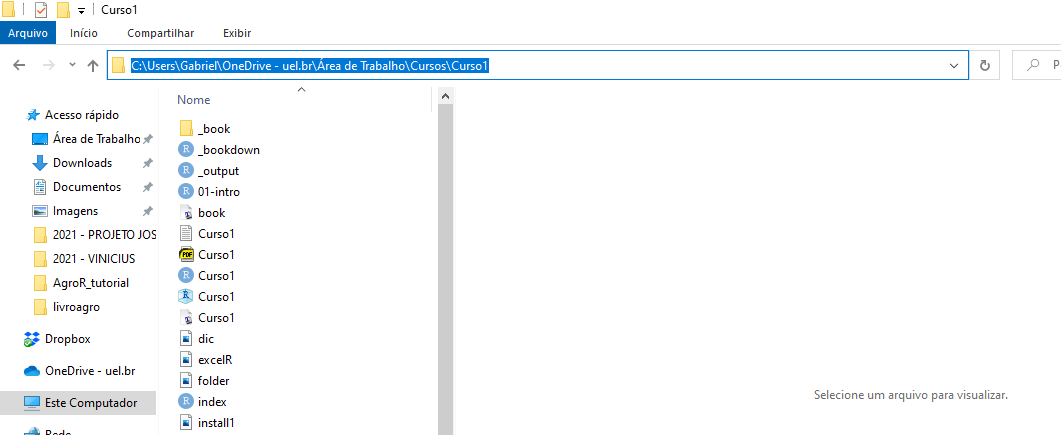
\includegraphics{pasta.png}
\caption{Figura 1: Especificando diretório de trabalho}
\end{figure}

A seguir, é necessário trocar as barras de ~para / ou adicionar mais uma \textbackslash{} (\textbackslash{} para \textbackslash) e colocar dentro do comando setwd e o diretório entre aspas.

Obs. O diretório abaixo é do \textbf{meu computador}!!!

\begin{Shaded}
\begin{Highlighting}[]
\FunctionTok{setwd}\NormalTok{(}\StringTok{"C:}\SpecialCharTok{\textbackslash{}\textbackslash{}}\StringTok{Users}\SpecialCharTok{\textbackslash{}\textbackslash{}}\StringTok{Gabriel Shimizu}\SpecialCharTok{\textbackslash{}\textbackslash{}}\StringTok{Dropbox}\SpecialCharTok{\textbackslash{}\textbackslash{}}\StringTok{SITE}\SpecialCharTok{\textbackslash{}\textbackslash{}}\StringTok{EXPERIMENTAL"}\NormalTok{)}

\DocumentationTok{\#\# ou}

\FunctionTok{setwd}\NormalTok{(}\StringTok{"C:/Users/Gabriel Shimizu/Dropbox/SITE/EXPERIMENTAL"}\NormalTok{)}
\end{Highlighting}
\end{Shaded}

Obs. \textbf{Sempre que for alterar a local da pasta, devemos alterar a localização do diretório!!!}

\hypertarget{opuxe7uxe3o-2-para-especificar-diretuxf3rio-1}{%
\subsection{Opção 2 para especificar diretório}\label{opuxe7uxe3o-2-para-especificar-diretuxf3rio-1}}

Atalho: ctrl+shift+h

Este comando irá buscar as \textbf{pastas} (não irá aparecer nenhum arquivo a menos que seja uma pasta). Buscar a pasta que contém o arquivo (Deverá saber onde fica, pois por esse método, o arquivo em extensão excel não irá aparecer, uma vez que o excel não é uma pasta)

Após encontrar, clicar em \textbf{``open''}. No console do R irá aparecer \textbf{setwd(localização)}, esta é a localização. Recomendo copiar e colar no \textbf{Source} do Rstudio

\hypertarget{conferir-se-o-arquivo-estuxe1-no-diretuxf3rio-especificado-1}{%
\subsection{Conferir se o arquivo está no diretório especificado}\label{conferir-se-o-arquivo-estuxe1-no-diretuxf3rio-especificado-1}}

\begin{Shaded}
\begin{Highlighting}[]
\FunctionTok{dir}\NormalTok{()}
\end{Highlighting}
\end{Shaded}

\hypertarget{importando-o-arquivo}{%
\subsection{Importando o arquivo}\label{importando-o-arquivo}}

\hypertarget{arquivo-separado-por-ponto-e-vuxedrgula-e-decimal-separado-por-vuxedrgula}{%
\section{Arquivo separado por ponto e vírgula e decimal separado por vírgula}\label{arquivo-separado-por-ponto-e-vuxedrgula-e-decimal-separado-por-vuxedrgula}}

\begin{Shaded}
\begin{Highlighting}[]
\NormalTok{dados}\OtherTok{=}\FunctionTok{read.csv2}\NormalTok{(}\StringTok{"DIC (CSV ponto e virgula).csv"}\NormalTok{)}
\NormalTok{dados}
\end{Highlighting}
\end{Shaded}

\hypertarget{arquivo-separado-por-vuxedrgula-e-decimal-com-ponto}{%
\subsection{Arquivo separado por vírgula e decimal com ponto}\label{arquivo-separado-por-vuxedrgula-e-decimal-com-ponto}}

\begin{Shaded}
\begin{Highlighting}[]
\NormalTok{dados}\OtherTok{=}\FunctionTok{read.csv}\NormalTok{(}\StringTok{"DIC (CSV virgula).csv"}\NormalTok{, }\AttributeTok{sep=}\StringTok{","}\NormalTok{)}
\NormalTok{dados}
\end{Highlighting}
\end{Shaded}

\href{https://agronomiar.000webhostapp.com/DIC\%20(CSV\%20virgula).csv}{Dados (Separado por vírgula)}

\href{https://agronomiar.000webhostapp.com/DIC\%20(CSV\%20ponto\%20e\%20virgula).csv}{Dados (Separado por ponto e vírgula)}

\hypertarget{tabulauxe7uxe3o-de-dados}{%
\chapter{Tabulação de dados}\label{tabulauxe7uxe3o-de-dados}}

Apesar da simplicidade em se tabular dados em uma planilha excel, a grande maioria dos acadêmicos tem dificuldade em se efetuar tal tarefa. Isso torna-se ainda pior, quando os mesmos precisam tabular de uma forma específica para um determinado \emph{Software}. Nesse contexto, o presente tutorial tem a finalidade de auxiliar os usuários de R a estruturar a planilha em excel de tal forma a facilitar as análises com ênfase em experimentação agronômica.

\begin{center}\rule{0.5\linewidth}{0.5pt}\end{center}

\textbf{O que não colocar em sua planilha!}

\begin{itemize}
\item
  Frequentemente é comum que os usuários de excel realizem cálculos de medidas de posição e dispersão, tais como média, variância, desvio-padrão, etc\ldots{} Entretanto, essas células preenchidas por tais estatísticas de nada contribuem para quem irá trabalhar com o R, muito pelo contrário, acabam gerando mais trabalho, visto que em alguns casos podem ocasionar confundimento no \emph{Software};
\item
  Deve-se evitar nomes de colunas muito extensos, pois operacionalmente digitar tais nomes pode gerar complicações futuras;
\item
  Nome de colunas sempre na primeira linha;
\item
  Evitar nome dos níveis do fator (Tratamentos) como numérico (1,2,3,4,\ldots), exceto quando os tratamentos são quantitativos;
\item
  Evitar pular células (Células em branco), a menos que tenha dados faltantes (parcelas perdidas).
\end{itemize}

\textbf{Monte a planilha da forma mais simples possível!!!}

\begin{center}\rule{0.5\linewidth}{0.5pt}\end{center}

\hypertarget{dic-unifatorial}{%
\section{DIC unifatorial}\label{dic-unifatorial}}

Experimentos em delineamento inteiramente casualizado só possuem o tratamento como fator. Dessa forma, em uma planilha, só necessitamos de \textbf{uma coluna de tratamentos e uma coluna de resposta}.

Quando há mais de uma variável resposta, pode-se adicionar as variáveis em cada coluna, lado a lado.

Abaixo, segue um imagem de como montar um arquivo em excel de um experimento em DIC com seis tratamentos e quatro repetições e o link para o download de um arquivo em excel (extensão .xlsx)

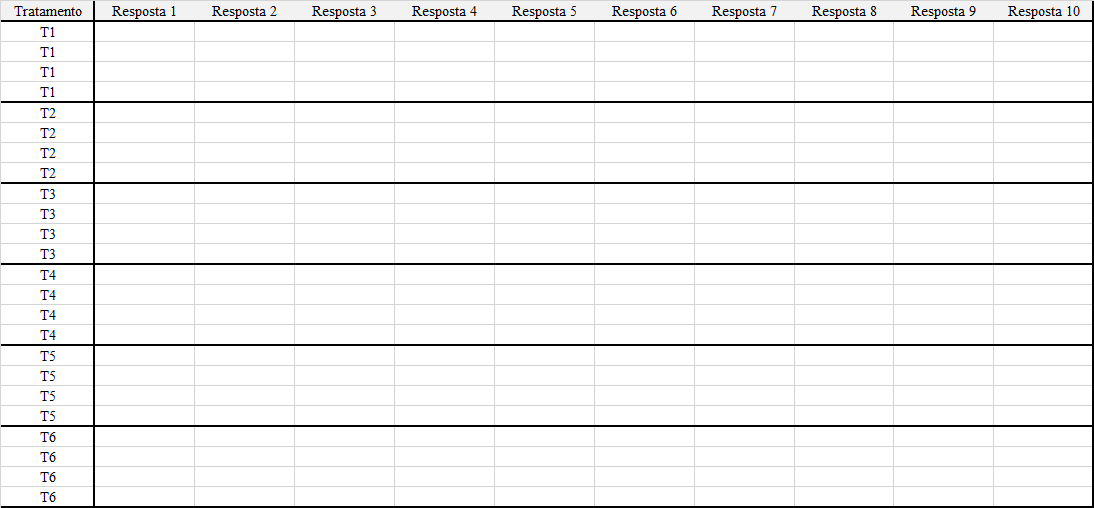
\includegraphics[width=10.41667in,height=\textheight]{dic.png}

\hypertarget{atalhos}{%
\chapter{Atalhos}\label{atalhos}}

Existem vários atalhos no Rstudio que facilitam a vida do usuário. Nos capítulos anteriores, vimos que o atalho ctrl+shift+h facilita a especificação do diretório de trabalho. Outros atalhos úteis, tais como o ctrl+shift+k para geração de relatórios via Rmarkdown, ou ctrl+shift+c para adicionar \# sobre as linhas são bastante populares entre os usuários.

A lista completa de atalhos do Rstudio podem ser acessadas utilizando o alt shift k.

Particularmente eu utilizo comandos como os já mencionados, o ctrl+shift+n para abrir uma nova guia R; ctrl+A para selecionar tudo; ctrl+shift+home ou ctrl+shift+end para selecionar da linha até o começo ou da linha até o fim, respectivamente; ctrl+S para salvar; ctrl+x para recortar; ctrl+z, ctrl+c e ctrl+v para voltar alteração, copiar e colar, respectivamente.

Assim como mencionado, existe diversos atalhos disponíveis no Rstudio, alguns pouco funcionais.

  \bibliography{book.bib,packages.bib}

\end{document}
